%% Placeholder for chapter on linear, quadratic, and geometric models

\section{Linear Programs: An Optimization Problem}

Also known as(a.k.a) (mathematical program") of the form

\begin{align*}
(arg)\,\,min_{x\in \Re^n}&c^Tx + d\,\,\,\text{("objective"function)}\\
s.t.\,\,\, &Ax = b\\
&Gx \leq h
\end{align*}

"Feasible" set(might not be good idea, but you can do this): $S = \{x|Ax = b, Gx \leq h \}$


\begin{itemize}
	\item $c\in \Re^n$, $d\in \Re$.
	
	\item $A\in \Re^{q\times n}$, $b\in \Re^q$, \begin{equation*}
	A = 
	\begin{bmatrix}
	\alpha^{(1)^T}\\
	...\\
	\alpha^{(q)^T}
	\end{bmatrix}
	\end{equation*}
	
	$<\alpha^{(i)}, x> =b_i$, $i\in \left[q\right]$
	
	\item $G\in \Re^{m\times n}$, $h\in \Re^m$
	
	\item If
	\begin{equation*}
	G = 
	\begin{bmatrix}
	g^{(1)^T}\\
	...\\
	g^{(q)^T}
	\end{bmatrix}
	\end{equation*}
	
	Then $<G^{(i)}, x>\leq h_i$, $i\in \left[m\right]$
	
\end{itemize}





\begin{align*}
p^* = min \,\,\, &c^Tx + d\\
s.t.\,\,\, &Ax = b\\
&Gx\leq h
\end{align*}

"optimal" value of program:

\begin{itemize}
	\item Lowest cost shoice amongst all feasible $x$.
	
	\item Possible here is no minimal choice
	
	\item possible no feasible choice
	
	\item $p^*\in \Re$
\end{itemize}


\begin{align*}
x^* = min \,\,\, &c^Tx + d\\
s.t.\,\,\, &Ax = b\\
&Gx\leq h
\end{align*}

$x^*$ "optimal" choice of optimization variable(or vector):

\begin{itemize}
	\item sometimes $x^*$ does not exist
	
	\item if exists, may or may not be unique
	
	\item $x^*\in \Re^n$
\end{itemize}


Let's consider an example:\\

During the The Second World War, the US army is considering how to make their soldiers have enough nutrients...\\

Different nutrients in different foods and daily requirement:\\


\begin{tabular}{|c|c|c|c|}
	\hline 
	Nutrients&Meat&Potatoes&Daily Requirement\\
	\hline  
	Carbohydates&40&200&400\\
	\hline  
	Protein&100&20&200\\
	\hline  
	Fiber&5&40&40\\
	\hline 
\end{tabular}\\

The price of meat and potatoes:\\



\begin{tabular}{|c|c|}
	\hline 
	Resources&cost/kg\\
	\hline  
	Meat &\$ 1\\
	\hline 
	Potatoes &\$ 0.25\\
	\hline 
\end{tabular}

$x_1$ denotes meat(kg) and $x_2$ denotes potatoes(kg).\\


Objective:

\begin{equation*}
x_1 + \frac{1}{4}x_2 = 
\begin{bmatrix}
1 & \frac{1}{4}
\end{bmatrix}
\begin{bmatrix}
x_1\\
x_2
\end{bmatrix}
\end{equation*}

Constrains:
\begin{align*}
40x_1 + 200x_2 &\geq 400\\
100x_1 + 20x_2 &\geq 200\\
5x_1 + 40x_2 &\geq 40\\
x_1 \geq 0\\
x_2 \geq 0
\end{align*}

$Gx\leq h \rightarrow$ 

\begin{equation*}
\begin{bmatrix}
-\frac{1}{5} & -1\\
-\frac{1}{8} & -1\\
-5 & -1\\
-1 & 0\\
0 & -1
\end{bmatrix}
\begin{bmatrix}
x_1\\
x_2
\end{bmatrix}\leq
\begin{bmatrix}
-2\\
-1\\
-10\\
0\\
0
\end{bmatrix}
\end{equation*}

\begin{figure}
	\centering
	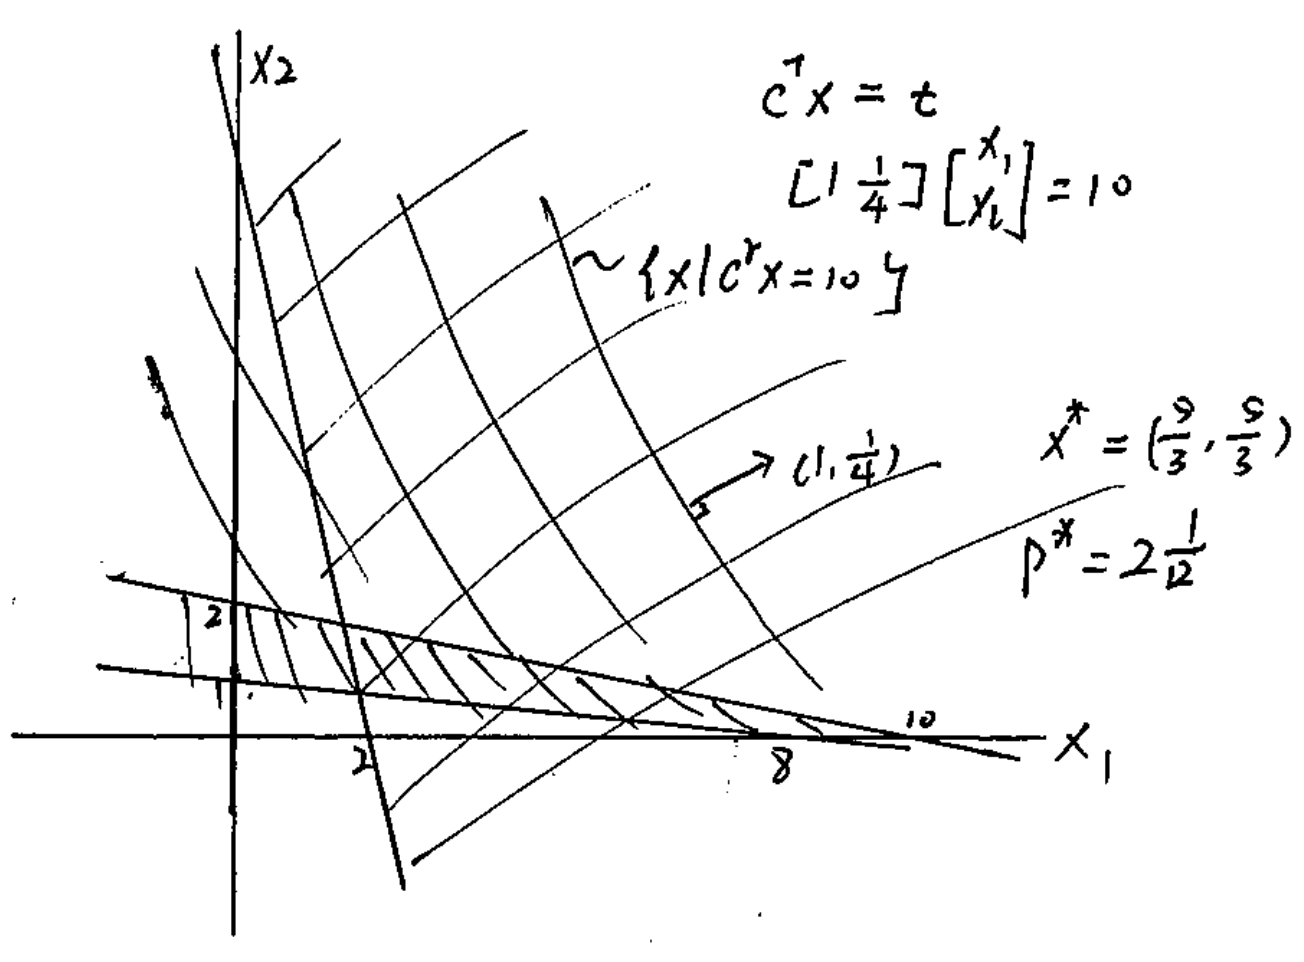
\includegraphics[width=2.1in,height=2.1in]{figures/ch06/figure5.png}
	%\caption{This is an inserted JPG graphic} 
	%\label{fig:graph} 
\end{figure}
